\documentclass[12pt]{../notes}

\usepackage{hyperref}

% Command for Questions
%\question{}

% Command for Notes
% \note{}

% Code to create a minipage where you can type in class notes. 
%%\begin{minipage}[l][2cm][c]{\textwidth}
\begin{comment}

\end{comment}
%%\end{minipage}


% Begin Document
%==============================================================================
\begin{document}
% Include the Title of the Handout
\ntitle{2.4: Simultaneous Inference and Important Considerations}

\question{(Hypothetical) Suppose you are searching for a relationship between a person's genetics and their likelihood to contract SARS-COV-2. You conduct individual t-tests between 1000 prominent genes (expressed vs non-expressed) and SARS-COV-2 infection/non-infection rates and find that 45 genes of them share a significant link with the likelihood of infection. Based on these results, what would you conclude about the 45 genes?}

\begin{minipage}[l][3cm][c]{\textwidth}
\begin{comment}
\note{Nothing. At least not from this test. We would have expected around 50 genes to have ``significant'' results just due to random chance. Without a multiple hypothesis adjustment, these results suggest that there is nothing different in the genetic expression of those who were infected and those who were not infected.}
\end{comment}
\end{minipage}


\section*{Regression Through the Origin}
Sometimes we wish to force the regression line to go through the origin (i.e. the point (0,0)), making the theoretical linear model become
\[
Y_i = \beta_1X_{i, 1} + \epsilon_i
\]


\nspace
\question{When might regression through the origin be a good idea?} 

\begin{minipage}[l][3cm][c]{\textwidth}
\begin{comment}
\note{\begin{itemize}
\item When the point (0,0) makes sense in the context of the data. 
\item When our sample size is small (avoiding an estimate of $\beta_0$ saves us one degree of freedom). 
\item If BOTH of the above conditions are not met, don't bother with regression through the origin. 
\end{itemize}
}
\end{comment}
\end{minipage}

\nspace
Cautions for regression through the origin:
\bi
\item $\sum_ie_i$ not necessarily equal to 0 (residuals might be unbalanced)
\item $R^2$ can be negative, giving it a nonsensical interpretation\
\ei

\newpage
\question{The following is a table of SAS output from a linear regression model fit with 16 observations. Observations that normally appear in the table but have been removed are denoted by a period. Please fill in all missing values}

\begin{figure}[H]
\centering
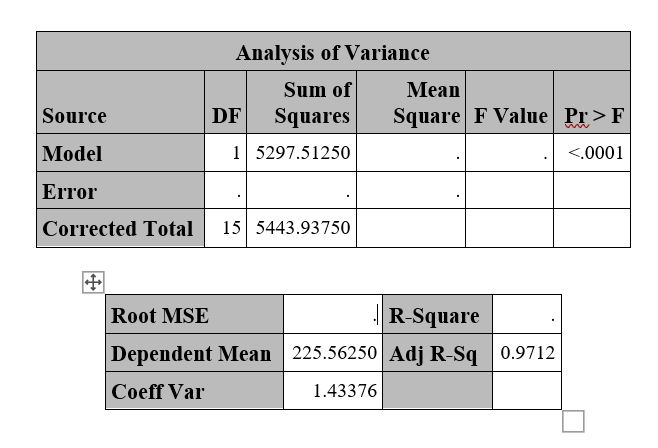
\includegraphics[width=0.85\textwidth]{../figures/module2/anova_table_pre.png}
\end{figure}

\begin{minipage}[l][12cm][c]{\textwidth}
\begin{comment}
\begin{figure}[H]
\centering
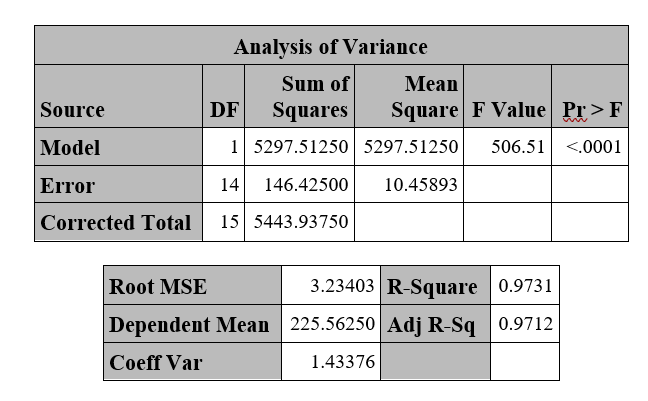
\includegraphics[width=0.85\textwidth]{../figures/module2/anova_table_post.png}
\end{figure}
\end{comment}
\end{minipage}

\section*{Extrapolation}
Extrapolation in linear regression is the use of your linear model to make a prediction for $Y$ that falls outside the range of observed response variables. When there are multiple X variables, this can include a situation where each individual X variable is technically within the range of observed observations, but the \textit{combination} of X variable inputs falls outside the range of the observed data. 


\nspace
\question{If I have created a linear model for prediction, isn't extrapolation the point?}

\begin{minipage}[l][3cm][c]{\textwidth}
\begin{comment}
\note{Slight extrapolations are usually not bad and even desirable. However, we do not know if the observed relationships between variables remains the same in unobserved territory. Abuse of this assumption may cause us to come to unreasonable conclusions.}
\end{comment}
\end{minipage}

Please check out the following story available at the following link:
\begin{center}
\url{https://www.nature.com/articles/431525a}
\end{center}

After reading this story: 

\question{Does this analysis provide convincing evidence that female Olympic sprinters will overtake male sprinters in 2156? Discuss why or why not.}

\begin{minipage}[l][3cm][c]{\textwidth}
\begin{comment}
\note{No. The extrapolation required for this conclusion lies far beyond the range of observed data. We can have no confidence that the trend observed over the past 100 years will continue for the next 150 years. }
\end{comment}
\end{minipage}


\question{What other interesting conclusions/observations might be made from these regression models fit to sprinter times?}

\begin{minipage}[l][5cm][c]{\textwidth}
\begin{comment}
\note{
\begin{itemize}
\item The percent variance in run times explained by the line is notably higher for the men than it is for the women. 
\item The range of available men's running times is notably longer than the availability of women's running times. 
\item (Possible): Is there anything notable about the times when the run times were notably lower than the prediction from the regression line?
\end{itemize}
}
\end{comment}
\end{minipage}

\nspace
\question{What, if anything, could be done to improve this analysis?}

\begin{minipage}[l][3cm][c]{\textwidth}

\end{minipage}


\begin{figure}[H]
\centering
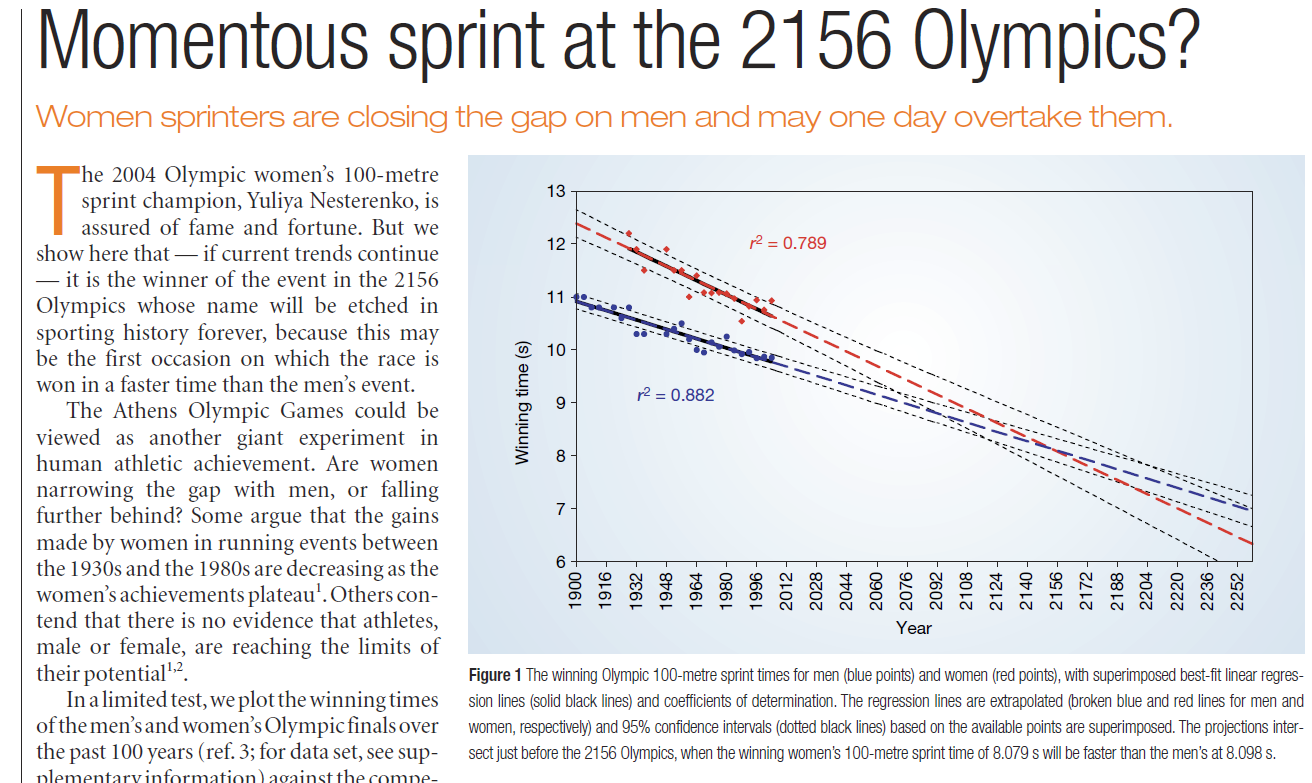
\includegraphics[width=\textwidth]{../figures/module2/sprint.png}
\end{figure}






% End the Document
%==============================================================================
\end{document}